\subsubsection{Presentation}
Stochastic Gradient Descent Classifier is an optimization technique to train other classification models, depending on chosen loss function it can be equivalent to an SVM or Logistic Regression models, it is particularly useful for large and sparse data.

\subsubsection{Defining Parameters}
The data for training and validating is already defined by the Data Preparation step (80\% train, 20\% validation).\\
Representative parameters for the model are \emph{max\_iter}, \emph{loss} and \emph{alpha}.
\begin{itemize}
    \item \underline{max\_iter}: stopping criterion, the algorithm can stop before, but never after this number of iterations.
    \item \underline{loss}: loss function, "hinge" is equivalent to a linear SVM, "log" is logistic regression.
    \item \underline{alpha}: regularization parameter (higher alpha, higher variance)
\end{itemize}
We trained \emph{alpha} over a logarithmically decreasing range [1, 0.1, 0.001...10**-7], \emph{max\_iter} over the range [10000, 100000] increasing 10000 per step, as well as across both "hinge" and "log" loss functions.\\
GridSearch was used with those ranges to determine best values for the hyperparameters, it was found to be alpha=0.01, loss=hinge, and  max\_iter=60000. \\
To improve the predictions, we regularize the data using a StandardScaler.
The training error and the validation error for each value allow us to plot a Complexity Curve, to select the optimal value fo the parameter.
Setting \emph{max\_iter}=60000, \emph{loss}="hinge", we plot the validation error across a range of values of \emph{alpha}
\begin{center}
    \captionsetup{type=figure}
    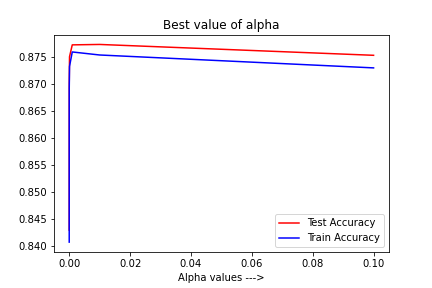
\includegraphics[width=250px]{SGD_complexity.png}
    \captionof{figure}{Complexity Curve: \emph{alpha} value for SVM}
\end{center}

\subsubsection{Model Evaluation}

With \emph{alpha}=0.01 we plotted a learning curve for the model as the sample size grows.
\begin{center}
    \captionsetup{type=figure}
    
\includegraphics[width=250px]{SGD Learning Curve.png}
    \captionof{figure}{Learning Curve for SVM}
\end{center}
This model shows extremely low bias and variance, and an increasing validation score as the data increases.\\
It is also important to note that this model only took a few seconds to train, which makes it much faster to train than the equivalent linear SVM, and much better suited for very large data.
